 \documentclass[twoside]{book}
\usepackage{geometry}
\usepackage{puzzles}



\geometry%{top=0.9in, bottom=0.9in,left=0.9in, right=0.9in, paperwidth=6in, paperheight=9in}
{top=0.9in, bottom=0.9in,inner=0.9in, outer=0.7in, paperwidth=6in, paperheight=9in}


\def\thetitle{Математические умопомрачилки} %заумки
\def\theauthor{Питер Винклер}
\hypersetup{
pdftitle={\thetitle},
pdfauthor={\theauthor},
pdfsubject={Математика}}


\makeindex[title=Указатель головоломок,intoc]

\makeatletter
\newcommand{\rindex}[2][\imki@jobname]{%
  \index[#1]{\detokenize{#2}}%
}
\makeatother


\begin{document}
%\pagestyle{empty}

\title{\thetitle}
\author{\theauthor\\
\\
Перевод с английского большой компанией}
\date{}
\maketitle

\thispagestyle{empty}

Предварительное издание предназначенное исключительно для отлова ляпов. 

Исправления слать по адресу 
\url{petrunin@math.psu.edu}.

\vfill

\chapter{Разминка}


\setlength{\epigraphwidth}{.80\textwidth}
\epigraph{Мозг (сущ.) --- приспособление, которым думают, что думают.}{--- Амброз Бирс (1842---1914), Словарь Сатаны}

Начнём с нескольких довольно простых задач для разминки мозга.
Для них почти не потребуется математики, только чуть-чуть логики.

\subsection*{Половина роста}

В каком возрасте средний ребенок достигает половины роста, до которого он дорастёт когда вырастит?

\subsection*{Шарики в мешочках}

Сколько нужно шариков, чтобы разложить в 15 мешочков так,
чтобы во всех мешочках было разное число шариков?

\subsection*{Степени двойки}

Сколько людей составляют \emph{дважды две пары двойняшек}?

\subsection*{Катящийся карандаш}

Карандаш с пятиугольным сечением имеет надпись на одной из пяти граней.
Предположим карандаш катится по столу.
С какой вероятностью он остановится надписью вверх?

\subsection*{Портрет}

Посетитель указывает на портрет и спрашивает, кто это. 
«Братьев и сестер у меня нет,» --- отвечает хозяин, --- «но отец этого человека --- сын моего отца».
Кто изображен на картине?

\subsection*{Странная последовательность}

Каким должен быть следующий символ в этой последовательности?

\begin{figure}[h!]
\centering

\includegraphics[scale=0.5]{pics/ZYXW}
\end{figure}

\subsection*{Параметр языка}

Для испанского, русского или иврита он равен 1.
Для немецкого --- 7.
Для французского --- 14.
Чему он равен для английского?

\subsection*{Вниманию параскаведекатриафобов}

Правда ли, что 13-е число месяца выпадет на пятницу чаще,
чем на любой другой день недели,
или это только так кажется?

\medskip

Теперь задачи посерьезнее.

\subsection*{Честная игра}

Как сделать равновероятный выбор 50 на 50, подбрасывая гнутую монету?

\subsection*{Кривые на картофелинах}

Даны две картофелины.
Докажите, что на их поверхностях можно нарисовать по замкнутой кривой так, чтобы обе кривые были идентичны как кривые в трехмерном пространстве.

\medskip

Завершим размнику тремя вероятностными задачами; в них потребуется \emph{кое-что} вычислять.

\subsection*{Победа на Уимблдоне}

В результате временных магических способностей вы попали в финал ... на Уимблдоне и играете против Серены Уильямс или Роджера Федерера ...
Однако магия не работает до победы.
На каком счёте лучше всего отказаться от магии, чтобы максимизировать свои шансы одержать победу?

\subsection*{Макаронные циклы}

100 концов 50 сваренных длинных макаронин произвольно разбиты на пары и соединены вместе.
Сколько циклов вы ожидаете так получить в среднем?

\subsection*{Рулетка для ротозеев}

Элвин приехал в Лас-Вегас на математическую конференцию и оказался в казино.
У него есть немного времени перед докладом и 105 долларов в кармане.
Он подошёл к рулетке и увидел, что на колесе 38 чисел (0, 00 и от 1 до 36).
Если поставить 1 доллар на какое-то число, то выигрываешь с вероятностью 1/38, получая 36 долларов (взамен своего доллара, который в любом случае забирает казино).
В противном случае, он просто теряет свой доллар.

У Элвина достаточно времени ровно на 105 таких однодолларовых ставок, и он решает так и поступить.
Оцените вероятность того, что Элвин окажется в плюсе?
Скажем, превысит ли эта вероятность 10\%?

\section*{Решения и комментарии}

\subsubsection*{Половина роста}

Родители маленьких детей знают ответ: два года!
(То есть между вторым и третьим днями рождения.)
Да, человечек растёт очень нелинейно.

Задача предложена Джеффом Стейфом из Университета Чалмерса в Швеции.

\subsection*{Шарики в мешочках}

Потребуется четырнадцать шариков.
Положите пустой мешочек в мешочек с одним шариком, 
далее второй мешочек в третий, с ещё одним шариком, затем третий в четвертый, с ещё одним шариком, и так далее.
Таким образом в $i$-ом мешочке будет $i-1$ шарик (и $i-1$ мешков).

Если вы не догадались засовывать мешочки в мешочки, или подумали, что так не честно, то вам потребуется $0 + 1 \z+ \z\dots \z+ 14 \z= 15 \times 7 \z= 105$ шариков.

Задача предложена Диком Плотцем из Провиденса, штат Род-Айленд.

\subsection*{Степени двойки}

Ответ восемь.
Четвёрка слов «дважды», «две», «пары», и «двойняшкa» натакливает на мысль что должно получиться $2^4 \z= 16$ человек.
Но двойняшка это только один человек.

Классическая задачка.

\subsection*{Катящийся карандаш}

Мой коллега Лори Снелл подловил меня на этой задачке.
А вы попались?
Похоже, что ответ должен быть $\tfrac15$, но поскольку $5$ нечётно, карандаш будет лежать гранью вниз и ребром вверх.
Таким образом, ответ $0$ или, если хотите, $\tfrac25$, в зависимости от вашего толкования термина \emph{вверх}, но уж всяко не $\tfrac15$.

Эта головоломка приведена в провокационной книге Чамонта Ванга \cite{wang}.

\subsection*{Портрет}

Это древняя загадка;
она приводится в классической книге Рэймонда Смаллиана \cite{smullyan}.

«Сын моего отца» может означать только самого хозяина, поскольку у него нет ни братьев ни сестёр.
А значит на портрете сын хозяина.

\subsection*{Странная последовательность}

Эту загадку переслал мне Кит Кохон, юрист из Агентства по охране окружающей среды.
Это начало алфавита в обратном порядке, то есть ZYXW, но буква Z повернутой на 90° (вправо или влево), и каждая последующая буква повернута на дополнительные 90°.
Следующим символом, следовательно, должна быть повернутая буква V, то есть < или >.

\subsection*{Параметр языка}

Ответ семь (seven).
Этот любопытный загадочный вопрос был придуман Тиной Кэрролл, аспиранткой Технологического института Джорджии,
и он слегка математический. 
Каждое число это первое многосложное натуральное число в данном языке.

\begin{addedbytheeditors}
Наверно лучше оставить вопрос про русский язык и лучше добавить языков знакомых многим нашим людям --- наверно турецкий=2, грузинский и финский=1, японский=6...
\end{addedbytheeditors}


\subsection*{Вниманию параскаведекатриафобов}

Удивительно, но правда.
Насколько мне известно, это было обнаружено Банкрофтом Брауном (профессор математики в Дартмутском колледже, как и автор этих строк), который привёл свои расчёты в журнале American Mathematical Monthly \cite{brown}.
На это мне указал мой нынешней коллега Дана Уильямс.

Не трудно проверить, что в 688 из 4800 месяцев в 400-летнем цикле григорианского календаря 13-е число выпадает на пятницу.
Воскресенье и среда приходятся по 687, понедельник и вторник по 685, а четверг и суббота только по 684.
Для этого нужно помнить, что годы, кратные 100, не являются високосными, если только (как 2000 год) они не делятся на 400.

Происхождение суеверия относительно пятницы 13-го обычно связывается с датой приказа, отданного французским королем Филиппом IV (Филиппом Красивым), о разгроме ордена храмовников.

Потренировавшись, можно научиться определить день недели любой даты в истории, даже учитывая прошлые календарные сложности
(по крайней мере, если вы человек, подобный внушающему восхищение Джону Конвею из Принстонского университета).
Для более ленивых смертных, ориентированных на настоящее время, полезно помнить, что в любом году
04.04, 06.06, 08.08, 10.10, 12.12, 09.05, 05.09, 07.11, 11.07 и последний день февраля выпадают на один и тот же день недели.
(Это еще легче запомнить, если вы играете в крэпс ежедневно с 9 до 5.)
Этот день недели --- среда для 2007 года;
перед невисокосным годом он сдвигается на один, и на два перед високосным.

\subsection*{Честная игра}

Подбросьте гнутую монету дважды в надежде получить орёл и решку.
Если сначала выпадет орёл, назовём результат «ОРЁЛ»;
если сначала выпадет решка, назовите его «РЕШКА».
Если получим две решки или два орла, то придётся повторить.

Мне напомнил об этой головоломке Тамаш Ленгель из Маккалестерского колледжа;
её решение приписывается покойному великому математику и пионеру компьютерных наук Джону фон Нейману и иногда называется «трюком фон Неймана».
Оно основано на том, что даже если монета гнутая, последующие броски являются (или по крайней мере должны быть) независимыми событиями.
Конечно же придётся предположить, что гнутая монета может приземлиться на любую сторону!

Если вы хотите минимизировать количество бросков, чтобы принять решение, вышеупомянутую схему можно улучшить. Например, если вы получаете орёл-орёл при первой паре бросков и решка-решка при второй, то можно назвать результат «ОРЛОМ» (конечно же решка-решка, за которым следует орёл-орёл, должен быть «РЕШКОЙ»).
Возможны и другие улучшения.
Статья Шербана Наку и Ювала Переса \cite{nacu-peres} выдавливает последнюю каплю из минимизации ожидаемого количества бросков, независимо от вероятностей получения орла и решки.

Кстати сказать, в последние годы, вопрос извлечения честных случайных битов из различных ненадёжных случайных источников становится важным в теории вычислений и является предметом многих научных работ и существенных прорывов.

\subsection*{Кривые на картофелинах}

Рассмотрите пересечение картофелин!
Другими словами, представьте каждая картофелина это призрак и воткните одну в другую.
Пересечение их поверхностей образует кривую на каждой из них; их и следует нарисовать.

Эту милую головоломку можно найти (среди прочего) в книге \cite{berlekamp-rodgers}.

\begin{addedbytheeditors}
Несмотря на столь простое решение, точная математическая формулировка задачи остаётся не ясной.

Пересечение поверхностей картофелин может быть фракталом не содержащим замкнутых кривых даже если сами поверхности гладкие.
В случае если поверхности гладкие, картофелины легко расположить так чтобы пересечение было гладкой замкнутой кривой.
Тоже можно сделать и при более слабых предположениях.

Однако, без дополнительных предположений вопрос остаётся открытым \cite{agol};
то есть неизвестно \emph{содержат ли две произвольные вложенные сферы в евклидовом пространстве пару конгруэнтных замкнутых кривых?} 
Более того, похоже, что вопрос откыт даже если обе вложенные сферы имеют конечную площадь.
Это предположение кажется разумным; как заметил Пер Александерсон,
«Я стараюсь не брать картофель с бесконечной поверхностью --- его слишком долго чистить.»
\end{addedbytheeditors}

\subsection*{Победа на Уимблдоне}

Кажется очевидным, что следует ...
(Вероятно, вы предпочтёте подавать, но если ваша подача такая же, как моя, то может быть лучше чтобы подавал ваш противник...)

Но подождите, не так быстро!
Эти решения дают три шанса что вам повезёт и вы выиграете, но можно добиться шести шансов...

Амит Чакрабарти из Дартмутского университета предложил следующее улучшение, основанное на идее, что традиционно полный счёт теннисного матча включает игровые очки всех партий и, если ...
Тогда, например, вы могли бы ...
Теория здесь (признаю, что сомнительная), заключается в том, что пока вы находились под вашим магическим заклинанием, ваш противник ... и легче совершит ошибку ...

\subsection*{Макаронные циклы}

Эта старинная задача, переданна мне коллегой из Дартмутского колледжа, Даной Уильямс.
Она эквивалентна «Игре ???» на странице 198 в книге Мартина Гарднера \cite{gardner1971}.
Вам нужно вычислить вероятность создания цикла на каждом этапе.
Тогда, используя \emph{линейность матожидания}, можно будет заключить, что ожидаемое число циклов это сумма полученных вероятностей.

При соединении $i$-го конца, вы берёте конец цепи, и из оставшихся $101 - 2i$ концов, только один (другой конец этой цепи) приводит к циклу.
Следовательно, вероятность того, что ваше $i$-е соединение добавит цикл, равна $1/(101 - 2i)$, и, следовательно, ожидаемое общее число циклов равно $1/99 + 1/97 + 1/95 +\dots + 1/3 + 1/1 = 2{,}93777485\dots$; меньше трех циклов!

Если у нас $n$ макаронин и $n$ большое число, то матожидание числа циклов близко к половине $n$-го гармонического числа, что примерно равно половине натурального логарифма $n$.

\subsection*{Рулетка для ротозеев}

Я услышал эту историю от Элвина Берлекэмпа на конференции
«Gathering for Gardner VII».
Позже она появилась в замечательном разделе «Головоломки» журнала Emissary \cite{berlekamp-buhle}, весна/осень 2006 года.

Игра в рулетку очень выгодна для казино (американский вариант ещё выгодней европейского в котором нет двойного нуля).
Ясно, что если повторять невыгодную ставку достаточно долго, то обычно окажитесь в проигрыше.
Каждая однодолларовая ставка приносит средний убыток в  $1 - (1/38) \times 36 = 1/19$ доллара, то есть примерно в пять центов.

Однако 105 это не так уж много!
Эльвину достаточно выиграть три раза, чтобы оказаться в плюсе.
В этом случае он получит 108\$ за свои 105\$.
Вероятность того, что он никогда не выиграет, составляет $(37/38)^{105} \approx 0{,}0608$;
выиграет ровно раз, $105 \times (1/38) \times (37/38)^{104} \z\approx 0{,}1725$;
и два раза, $105 \times (104/2) \times (1/38)^2 \times (37/38)^{103} \approx 0{,}2425$.
Таким образом, вероятность оказаться в плюсе равна единице минус сумма этих трёх значений, что составляет $0{,}5242$ --- больше половины!

Конечно же это не означает, что Эльвин может дурачить Лас-Вегас.
Ведь когда ему не удается получить три победы, он теряет как минимум 33 доллара, намного больше, чем 3 доллара прибыли, которую он получает, когда выигрывает ровно три раза.
(А проигрывает он в 43\% случаев???)
В среднем Эльвин потеряет $105 \times (1/19) \approx 5{,}53$ долларов.

Рассмотрим более жёсткий вариант этой задачи.
Предположим, что у Эльвина есть 255\$, но ему нужно 256\$ чтобы зарегестрироваться на математической конференции.
Тогда лучше всего сделать ставку в 1\$, затем 2\$, затем 4\$, 8\$, 16\$, 32\$, 64\$ и, наконец, 128\$ на красное (или чёрное).
Первый раз, когда он выигрывает, он получает в два раза больше своей ставки и сразу же прекращает, имея ровно те 256\$, которые ему нужны.
Он терпит неудачу только если проигрывает все 8 ставок (и все свои деньги), что происходит с вероятностью только $(20/38)^8 < 0{,}006$.

Попробуйте сами если вам не страшно потерять 255\$.
Вы можете посетить казино и в 99\% случаев останетесь в плюсе.
Потом лучше бросить играть в азартные игры, очень рекомендую.

\chapter{Полёт фантазии}

%Кноп

\setlength{\epigraphwidth}{.80\textwidth}
\epigraph{Не стоит доверять глазам, когда разыгралось воображение.
}{--- Марк Твен (1835---1910), Янки при дворе короля Артура}

Следующие головоломки потребуют разработки \emph{плана},
и иногда вам придётся напрячь воображение!

\subsection*{Любовь в Клептопии}\rindex{Любовь в Клептопии}\label{Любовь в Клептопии}

Ян влюбился в Марию (по интернету), и он хочет послать ей обручальное кольцо.
Однако они живут в Клептопии, стране, где всё отправленное по почте будет неминуемо украдено, если только не отправлено в ящике, запертом на навесной замок.
У Яна и Марии много замков, но ни у кого из них нет ключа к замку другого.
Как им переслать кольцо?

\subsection*{Черви и вода}\rindex{Черви и вода}\label{Черви и вода}

Лори надоело, что черви забираются к ней на кровать.
Она поставила ножки кровати в вёдра с водой;
поскольку черви не умеют плавать, они не могут добраться до кровати по полу.
Однако теперь они ползут вверх по стенам и по потолку, и падают на кровать сверху.
Фу!

Как защититься от червей?

\parit{Примечания.}
Можно попробовать соорудить навесную конструкцию над кроватью.
Для того чтобы предотвратить падение червей на навес,
их дальнейшее проползание по навесу
и падение на кровать, возможно, стоит сделать жёлоб вокруг навеса и наполнить его водой.
Но ведь тогда черви смогут упасть на край жёлоба.
Хм...

\subsection*{Проверка страусиных яиц}\rindex{Проверка страусиных яиц}

В преддверии рекламной кампании страусиной ферме нужно проверить яйца своих страусов на прочность.
В мировой практике прочность определяют по самому высокому этажу Эмпайр-стейт-билдинга, с которого можно сбросить яйцо так, чтобы оно не разбилось.

Официальный инспектор фирмы, Оскар, понимает, что если он возьмёт с собой в Нью-Йорк одно яйцо,
то для определения прочности придётся (возможно) бросить его с \emph{каждого} из 102 %101???
этажей, начиная с первого.
А что если он возьмёт \emph{два} яйца?
Сколько бросков ему потребуется в худшем случае?

%\begin{addedbytheeditors}
%\textbf{Редакторам:}
%Тут возникает проблема с американской и русской нумерацией этажей + похоже, что Уинклер считает, что нет смысла бросать яйцо с нулевого этажа.
%\end{addedbytheeditors}


\subsection*{Опасная картина}\rindex{Ненадежная картина}

Требуется повесить картину за шнур, прикреплённый к раме.
Если это сделать, как обычно, перекинув шнур через два гвоздя (как показано на рисунке), и один из гвоздей выпадет, то картина останется висеть на другом гвозде (хотя и накренится).

Можно ли повесить картину так, чтобы она упала в случае, если выпадет \emph{любой} из двух гвоздей?

\begin{figure}[h!]
\centering
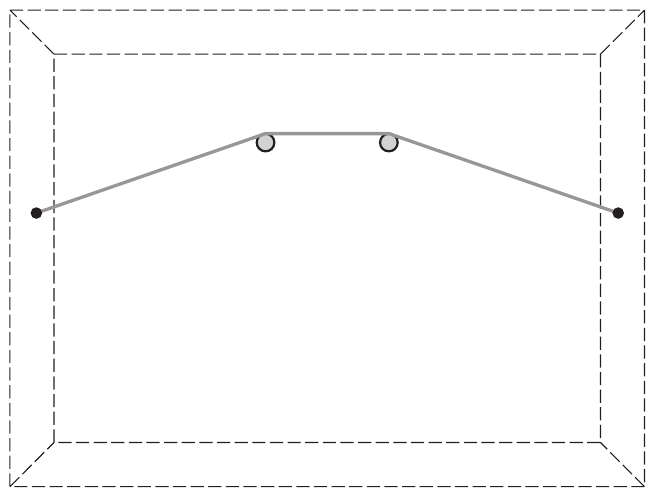
\includegraphics[scale=0.5]{pics/kartina1}
\caption{Эта картина останется висеть если выпадет любой из гвоздей.}
\label{pic:kartina1}
\end{figure}

\subsection*{Замок с дефектом}\rindex{Замок с дефектом}\label{Замок с дефектом}

Кодовый замок имеет три диска, с положениями пронумерованными от 1 до 8.
У замка есть дефект: чтобы его открыть, достаточно правильно выставить два числа из трёх.
Какое минимальное число (трёхзначных) комбинаций достаточно набрать, чтобы наверняка открыть замок?

\parit{Примечания.}
Есть много способов проделать это $64$-мя тестовыми комбинациями, например, можно перебрать все возможные варианты первых двух дисков или проверить все комбинации, сумма значений которых кратна 8.
Однако каждая тройная комбинация покрывает $22$ возможных случаев, а всего комбинаций $8^3 = 512$.
Поэтому в принципе могло бы хватить и $\lceil 512/22 \rceil = 24$ комбинаций.
То есть истина лежит где-то между $24$ и $64$; вопрос --- где?

\subsection*{Альтернативные кубики}\rindex{Альтернативные кубики}

 
Можно ли изготовить такую пару игральных кубиков, чтобы их суммы вели себя так же, как у пары обычных кубиков?
То есть должно быть два способа выбросить 3, шесть способов выбросить 7, один способ выбросить 12 и так далее.
У кубиков должно быть по шесть граней, и на каждой грани должно быть указано положительное целое число.

\subsection*{Совпадение монет}\rindex{Совпадение монет}

Сонни и Шер\footnote{Сонни и Шер --- популярный в 1970-е годы американский поп-рок дуэт Сонни Боно и его супруги Шер.\pr} играют в следующую игру.
В каждом раунде бросается честная монета.
Перед броском Сонни и Шер одновременно объявляют свои предположения о результате броска.
Они выигрывают раунд, если оба угадали правильно.
Требуется максимизировать долю выигранных раундов, предполагая, что игра идёт долго.

Пока что ответ очевиден --- 50\%: Сонни и Шер договариваются о последовательности предположений (например, всегда говорить «орёл»).
Очевидно, что лучшего им не добиться.

Однако перед началом игры игрокам сообщается, что Шер получит результаты всех бросков монеты заранее, прямо перед первым броском!
У неё есть возможность обсудить стратегию с Сонни заранее, но как только она получит данные о бросках, возможности передавать информацию больше не будет.
Возможно ли им добиться 70\%-й доли выигрышей?

\subsection*{Имена в ящиках}\rindex{Имена в ящиках}\label{Имена в ящиках}

Имена ста заключённых помещают в сто деревянных ящиков, по одному в каждом;
ящики расставляются в ряд на столе в комнате.
Заключённых приводят в комнату поочерёдно;
каждому позволяется заглянуть не более чем в 50 ящиков,
затем он должен покинуть комнату, оставив её в точно том же состоянии, как до прихода, и дальнейшее общение невозможно.

У заключённых есть возможность спланировать свою стратегию заранее, и им это понадобится --- если хотя бы один заключённый не найдёт своё имя, то казнят всех.
Найдите стратегию, вероятность успеха которой превысит 30\%.

\parit{Примечания.} Если каждый заключённый откроет случайный набор из 50 ящиков, то вероятность выжить составит незавидные
\[(\tfrac12)^{100}\z\sim 0{,}0000000000000000000000000000008.\]
Но они могут поступить и хуже --- если все откроют одни и те же 50 ящиков, то их шансы упадут до нуля.
Но тридцать процентов уж совсем недостижимы...
Очень хорошо --- вы поняли задачу!

\section*{Источники и решения}

\subsubsection*{Любовь в Клептопии}

Эта головоломка приводится в книге Саймона Сингха \cite{singh};
я узнал её от Кэролайн Калдербэнк, дочке пары математиков Ингрид Добеки и Роба Калдербэнка.
В решении Кэролайн, Ян отправляет Марии ящик с кольцом внутри, навесив на него один из своих замков.
По получении Мария навешивает свой собственный замок на ящик и отправляет её назад с обоими замками.
Когда Ян получает ящик, он снимает свой замок и отправляет ящик опять Марии; вуаля!

Это решение не просто игра;
на нём основан обмен ключами шифрования в протоколе Диффи — Хеллмана, историческим прорывом в криптографии.

В зависимости от предположений, возможны и другие решения.
Моё любимое было предложено компанией участников конференции
«Ga\-the\-ring for Gardner VII», включая оригамиста Роберта Лэнга.
Для этого Ян должен найти замок, ключ от которого имеет большое отверстие, или по крайней мере, отверстие, которое может быть достаточно увеличено сверлением, чтобы ключ мог быть нацеплен за дужку другого замка.
Ян использует этот второй замок, с упомянутым ключом на его дужке, чтобы запереть пустой ящичек, которую он отправляет Марии.
По прошествии времени, достаточном для пересылки (или возможно, после электронного подтверждения от Марии), он отправляет кольцо в другом ящике, запертой первым замком.
Когда Мария получает ящик с кольцом, она открывает её ключом, прикреплённым к первому ящичку, и получает кольцо.

\subsubsection*{Черви и вода}

Это скорее инженерная головоломка, чем математическая.
Она пришла ко мне от Балинта Вирага из Массачусетского технологического института.

Лори действительно может защититься от червей свесив с потолка большой навес, выходящий далеко за кровать.
Но навес должен загибаться внутрь под себя по краям, создавая кольцевой жёлоб, заполненный водой.
(Поперечный разрез навеса показан на рис. \ref{pic:chervi}.)

\begin{figure}[h!]
\centering
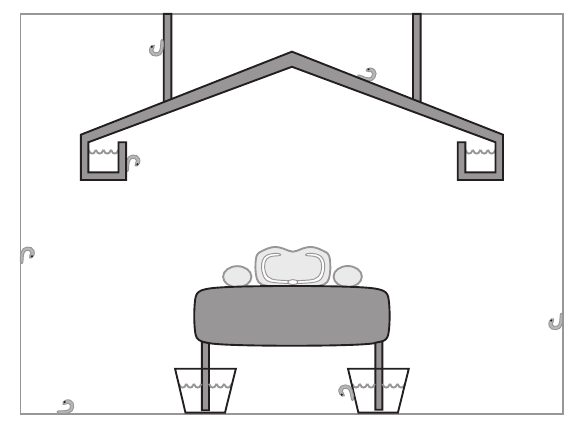
\includegraphics[scale=0.5]{pics/chervi}
\caption{Поперечный разрез Лори в защищённой от червей кровати.}
\label{pic:chervi}
\end{figure}

Если у червей нет способа проникнуть в спальню сверху, то Лори может защититься, обведя комнату по краю жёлобом с водой.

\subsubsection*{Инспекция страусиных яиц}

Вариант этой задачи появился в замечательной книге Джозефа Д. Э. Конхаузера, Дэна Веллемана и Стэна Уэгона \cite{konhauser-velleman-wagon}.

Часто полезно считать данное число (в нашем случае 102) переменной, даже если в конечном счёте нас интересует лишь одно значение.
Пусть $f(k)$ --- максимальное число этажей, которые можно проверить не более чем за $k$ бросков, имея вначале два яйца.
Таким образом, $f(1) = 1$ (прочность яйца может быть $0$ или $1$).
Предположим, что Оскару разрешено сделать $k$ бросков, и он делает первый с $n$-го этажа.
Если яйцо разбилось, то Оскару придётся бросить единственное оставшееся яйцо с 1-го этажа, затем с 2-го и так далее до $(n-1)$-го в худшем случае;
так что $n = k$ это наилучший вариант.
Если яйцо пережило падение с $k$-го этажа, то придётся проверить все этажи выше оставшимися $k-1$ броском (используя два яйца).
Следовательно, $f(k - 1) + k$ это максимальное число этажей, которые можно обработать,
и мы получили рекурсию $f(k) = f(k - 1) + k$.

Прямым вычислением получаем, что $f(2) = 3$, $f(3) = 6$, $f(5) = 10$ и так далее; в общем случае $f(k)$ равно сумме чисел от $1$ до $k$.
Поскольку таких чисел $k$, а их среднее равно $(k + 1)/2$, их сумма (иногда называемая «$k$-ым треугольным числом»), составляет $k(k + 1)/2$.
Первое значение $f(k)$, достигающее 102, это $f(14) = 14 \times 15/2 = 105$, то есть в худшем случае Оскару понадобится $14$ бросков.
Рекурсия указывает и на то как это сделать;
в нашем случае, трёхэтажный запас позволяет Оскару сбросить первое яйцо с одиннадцатого, двенадцатого, тринадцатого или четырнадцатого этажа.
Любой другой вариант может потребовать лишнего броска.

Давайте посмотрим, что происходит с тремя яйцами.
Определим $g(k)$ как максимальное число этажей, которые можно обработать $k$ бросками, начиная с трёх яиц.
Теперь Оскару нужно обработать $g(k \z- 1)$ этажей выше уровня первого броска, если яйцо переживёт падение;
или же $f(k - 1)$ этажей ниже этого уровня (тот же $f$, что и выше), потому что теперь у него лишь два яйца.
Получаем новую рекурсию: $g(k) = g(k-1) + 1 + (k - 1)k/2$, что даёт $g(2) = 3$ (пока без улучшений), но $g(3) = 7$.
В общем случае получаем $g(k)=k(k^2+5)/6$ и наименьшее значение $k$, для которого 
$g(k)\ge 102$, равно $9$.
То есть, если у Оскара есть три яйца,
то ему потребуется максимум девять бросков чтоб обработать Эмпайр-стейт-билдинг.

В общем случае, если $k$ велико, то число этажей, которые можно обработать, имея вначале $m$ яиц, равно $k^m/m!$ плюс члены низших порядков.
Отсюда следует, что с $m$ яйцами и небоскрёбом в $n$ этажей, где  $n$ намного больше $m$, число бросков, необходимых в худшем случае, будет около $(m!\times n)^{1/m}$.

\subsubsection*{Опасная картина}

Эту интересную головоломку предложил Джулио Дженовезе, аспирант в Дартмуте, который узнал её из нескольких источников в Европе.

Один из способов повесить картину изображён на рис. \ref{pic:kartina2}, с зазором, чтобы можно было в нём разобраться.
Шнур проходит над первым гвоздём,
далее идёт петля вокруг второго,
проходит опять над первым гвоздём, и затем снова петля вокруг второго гвоздя, но на этот раз с половинным поворотом.

\begin{figure}[h!]
\centering
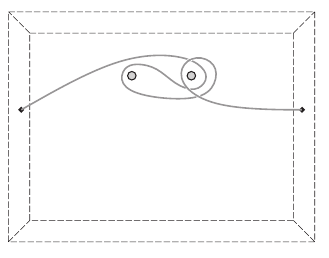
\includegraphics[scale=1]{pics/kartina2}
\caption{Эта картина упадёт если выскочит любой из двух гвоздей.}
\label{pic:kartina2}
\end{figure}

Существуют также некоторые нетопологические решения: например, можно сдавить петлю между двумя близко расположенными гвоздями, предполагая, что ширина головки гвоздя не намного больше толщины шнура.
Но зачем полагаться на трение, когда можно использовать математику?

\begin{addedbytheeditors}
Попробуйте повесить картину на $n$ гвоздей так, чтобы она упала если выскочит любой из них.
А можно ли повесить так, чтоб картина осталась висеть при выпадании одного гвоздя, но падала при выпадании двух?
Хороший обзор подобных задач дан в \cite{demaine2014}, но он не включает результата из \cite{gartside-greenwood}, дающего наилучий способ решения задачи с $n$ гвоздями (без заузливания шнура).
\end{addedbytheeditors}

\subsubsection*{Дефективный кодовый замок}

Этот шедевр комбинаторики достался мне от Амит Чакрабарти из Дартмута;
он был предложен Восточной Германией для Международную математическую олимпиаду 1988 года.

Задачи такого рода лучше решать геометрически.
Пространство всех комбинаций представляет собой комбинаторный куб $8 \times 8 \times 8$.
Каждый раз, когда мы проверяем точку куба, мы вычёркиваем все точки на трёх её координатных линиях.

Представив задачу таким способом, должно быть видно, что лучший способ вычеркнуть все точки это брать все тестовые точки в двух противоположных осьмушках $4 \times 4 \times 4$ нашего куба.
Так можно догадаться до следующего решения.

Давайте проверим все комбинации с числами из $\{1, 2, 3, 4\}$, сумма которых кратна $4$.
Их всего шестнадцать, так как если вы выбираете числа на первых двух (или любых двух) дисках, то число на третьем определяется однозначно.
Теперь попробуем те же комбинации, добавив $(4,4,4)$, то есть, добавив $4$ к каждому из трёх чисел;
их ещё $16$, и мы утверждаем, что вместе эти $32$ комбинации вычёркивают все.

Проверка довольно лёгкая.
Правильная комбинация должна иметь либо два (или более) числа из $\{1, 2, 3, 4\}$, либо два или более числа из  $\{5, 6, 7, 8\}$.
В первом случае положение третьего диска единственно (это число в правильной комбинации может не входить в $\{1, 2, 3, 4\}$), так что получена тройка среди первых $16$ тестовых комбинаций.
Второй случай аналогичен.

А вот способ Амита (есть и другие), объясняющий, что нельзя обойтись $31$-й или менее тестовой комбинацией.
Предположим, что $S$ --- это покрытие, и $|S| = 31$.
Пусть $S_i = \{\,(x, y, z) \z\in S : z = i\,\}$ будет $i$-м уровнем $S$.

Рассмотрим три множества:
$A=\{1, 2, 3\}$,
$B = \{4, 5, 6, 7, 8\}$,
и $C \z= \{2, 3, 4, 5, 6, 7, 8\}$.
По крайней мере, один уровень $S$ должен содержать три или меньше точек;
можно считать, что это $S_1$, и $|S_1| = 3$.
(Если $|S_1| \le 2$, то дойти до противоречия ещё проще.)
Точки $S_1$ должны лежать в некотором $3 \times 3 \times 1$ подкубе;
можно считать, что они лежат в $A \times A \times {1}$.

Заметим, что $25$ точек в $B \times B \times \{0\}$ должны быть вычеркнуты точками, не входящими в $S_1$.
Никакие две из них не могут быть вычеркнуты одной точкой в $S$.
Следовательно, $S - S_1$ содержит подмножество $T$ размером $25$, которое лежит в подкубе $B \times B \times C$.
Теперь рассмотрим множество $P = \{\,(x, y, z) : z \in C, (x, y, 1) \notin S_1 , (x, y) \notin B \times B\,\}$.
Легко подсчитать, что $|P| = (64-3-25) \times 7 = 252$.
Точки в $P$ не вычёркиваются $S_1$, и каждая точка в $T$ может вычеркнуть не более $3 + 3 = 6$ точек в $P$. Следовательно, есть по крайней мере $252 - 6 \times 25 = 102$ точки в $P$, которые должны быть вычеркнуты точками в $S - S_1 - T$.

Однако осталось всего $|S - S_1 - T | = 31 - 3 - 25 = 3$ тестовых точек, и каждая из них вычёркивает ровно $22$ точки.
Поскольку $22 \times 3 = 66 \z< 102$, приходим к противоречию. 

\subsubsection*{Альтернативные кубики}

Эта задача настолько известна, что у её решение есть имя: «кубики Шихермана».
В заметке Мартина Гарднера 1978 года \cite{gardner1978} или в ego книге \cite{gardner1989} можно узнать об их открытии полковником Джорджем Шихерманом, сейчас проживающим в Уэйсайд, Нью-Джерси.
Единственная пара кубиков Шихермана имеет метки $\{1, 3, 4, 5, 6, 8\}$ и $\{1, 2, 2, 3, 3, 4\}$.

Возможно, вы нашли ответ перебором, и это вполне подходящий способ решения.
Однако есть и другой способ, иллюстрирующий мощный математический инструмент --- \emph{производящие функции}.

Идея в том, чтоб сопоставить кубику многочлен от переменной $x$, в котором коэффициент при $x^k$ равен числу граней кубика с меткой $k$.
Обычный кубик, например, будет соответствовать многочлену $f(x) = x \z+ x^2 \z+ x^3 \z+ x^4 \z+ x^5 \z+ x^6$.

Ключевое наблюдение заключается в том, что результат броска двух (или более) кубиков представлен произведением их многочленов.
Например, если мы бросаем два обычных кубика, то коэффициент $x^{10}$ в произведении (то есть в $f(x)^2$) есть число способов выбора двух членов из $f(x)$, произведение которых равно $x^{10}$ ---
это $x^4 \times x^6$, $x^5 \times x^5$ и $x^6 \times x^4$; они представляют три способа получить сумму $10$.

Следовательно, если $g(x)$ и $h(x)$ --- многочлены наших кубиков, то $g(x) \times h(x) = f(x)^2$.
Многочлены, как и числа, единственным способом разлагаются на простые сомножители;
многочлен $f(x)$ разлагается как $x(x + 1)(x^2 + x + 1)(x^2 - x + 1)$.
Чтобы получить произведение $g(x)$ и $h(x)$ равное $f(x)^2$, нам нужно взять каждый из этих $4$ сомножителей и добавить по одной его копии в $g(x)$ и в $h(x)$, или же две его копии в один либо в другой.
Но есть следующие ограничения:
в полученных многочленах $g(x)$ и $h(x)$ не может быть свободных членов (это бы означало, что некоторые стороны помечены нулём);
не допускаются отрицательные коэффициенты;
также сумма коэффициентов в каждом из этих многочленов должна равняться 6.


Единственный решение (кроме $g(x) = h(x) = f(x)$) это
\[g(x)
=
x(x + 1)(x^2 + x + 1)
=
x + 2x^2 + 2x^3 + x^4\]
и
\[h(x)
=
x(x + 1)(x^2 + x + 1)(x^2 - x + 1)^2
=
x + x^3 + x^4 + x^5 + x^6 + x^8,\]
или наоборот.

Мы всё ещё использовали перебор, но таким методом можно решать задачи посложнее.
Во-первых, можно придумать альтернативы для пары восьмигранных игральных костей, пронумерованных от $1$ до $8$ (есть три альтернативных варианта), или для бросания трёх обычных кубиков (много способов).

Читателям, которые хотят поглубже изучить эту тему, стоит обратиться к отличной статье Джо Галлиана и Дейва Русина \cite{gallian-rusin}.

\subsubsection*{Совпадение монет}

Эту задачу предложил мне Одед Регев, из Техниона, в Израиле.
Сонни и Шер могут выиграть более чем в 2/3 случаев.
Для этого разделим последовательность бросков на блоки по три.
Перед каждым блоком Шер \emph{оповещает} Сонни, будут ли в следующем блоке в основном орлы или решки;
если первое, Сонни говорит «ООО» в этом блоке; если второе, то «РРР».

Но как Шер передать эту информацию?
Чаще всего Сонни ошибается (в точности) раз в блоке.
Перед этим броском Шер говорит «О», сообщая, что в следующем блоке будут в основном орлы, и «Р» в противном случае.
Для двух других бросков в текущей тройке Шер даёт правильный ответ (вместе с Сонни), гарантируя две из трёх побед.
Если случится, что Сонни может угадать все три броска в текущей тройке,
то один раз --- скажем на последнем броске, Шер действует, как описано выше, даже если это стоит им потери одной победы.
Таким образом, после первого блока Сонни и Шер будут набирать две победы из трёх, когда блок состоит из двух орлов и одной решки или двух решек и одного орла.
Когда блок состоит полностью из орлов или полностью из решек (что происходит с вероятностью 1/4), они получают две победы из трёх в половине случаев и три из трёх в остальной половине.
Значит доля успеха составит $3/4 \times 2/3 + 1/4 \times 5/6 = 17/24 > 70.8\%$.
Обратите внимание, что даже в наихудшем случае (например, если последовательные орлы и решки выбираются противником, а не случайны) этот метод гарантирует долю успеха хотя бы $2/3$.

Оливье Госснер, Пенелопа Эрнандес и Абрахам Нейман \cite{gossner} доказали, что с более сложными версиями этой схемы Сонни и Шер могут приблизиться к любой доле успеха равной $x$, где $x$ --- единственное решение уравнения
\[-x \log_2 x - (1 - x) \log_2 (1 - x) + (1 - x) \log_2 3 = 1,\]
и лучшего добиться нельзя.
Более того, это утверждение остаётся верным независимо от того, случайны ли броски монеты или нет!
Поскольку это значение $x$ составляет около $0{,}8016$, Сонни и Шер могут на самом деле добиться победы более чем в $80\%$ случаев, даже если оппонент играет против них.

\subsubsection*{Имена в ящиках}

У этой головоломки короткая, но увлекательная история.
Она придумана датским специалистом по информатике Петером Бро Милтерсеном;
её версия появилась в завоевавший широкое признание статье, написанной им и Анной Галь \cite{gal-miltersen}.
Однако Милтерсен не знал  решения, пока его коллега Свен Скиум не указал ему на это во время обеда.
В конечном итоге головоломка дошла до меня (в несколько усложнённой форме) через Дорит Ахаронов.

Чтобы её решить, заключённые должны сначала договориться о случайном соответствии ящиков со своими именами.
(Это сделает невозможным разложить имена в ящиках так, чтобы помешать протоколу, описанному ниже.)
Попадая в комнату, каждый заключённый проверяет свой собственный ящик (то есть ящик, с которому соответствует его имя).
Затем он заглядывает в ящик, соответствующий имени, которое он только что нашёл,
затем в ящик, соответствующий имени, найденному во втором ящике, и так далее, пока он не найдёт своё собственное имя или не откроет 50 ящиков.

Вот такая стратегия, но почему она работает?
Соответствие, между именем владельца ящика и именем, найденном в его ящике, представляет собой перестановку из 100 имён, выбранную равномерно случайным образом из набора всех таких перестановок.
Каждый заключённый идёт по циклу перестановки, начиная со своего имени.
Если цикл не длиннее 50, то он находит своё имя.
Если перестановка не длинней 50, то это сработает для всех, и заключённые будут спасены.

Вероятность того, что равномерно случайная перестановка чисел от $1$ до $2n$ не содержит ни одного цикла длиной более $n$, равна по крайней мере, $1$ минус натуральный логарифм от $2$, что составляет около $30,6853\%$.

Чтобы увидеть это, положим $n < k \le 2n$ и сосчитаем перестановки, имеющие цикл $C$ длиной ровно $k$.
Есть $\binom{2n}k$ способов выбрать имена в этом цикле, $(k - 1)!$ способов упорядочить их в $C$
и $(2n - k)!$ вариантов перестановки остальных имён;
произведение этих чисел равно $(2n)!/k$.
Поскольку в данной перестановке не более одного $k$-цикла, вероятность того, что такой имеется, в точности равна $1/k$.
Значит вероятность отсутствия длинного цикла равна
\[1-\frac{1}{n}-\frac{1}{n+1}-\dots-\frac{1}{2n}=1-H_{2n}-H_n\]
где $H_m$ --- сумма обратных чисел первых $m$ положительных целых чисел, что приблизительно равно $\ln m$.
Таким образом, наша вероятность будет близка к $1 - \ln 2n + \ln n = 1 - \ln 2$, на самом деле всегда чуть больше этого значения.
Для $n = 50$ мы получаем, что заключённые выживают с вероятностью $31,1827821\%$.
Недавно Юджин  Кертин и Макс Варшауэр \cite{curtin-warshaue} показали, что это решение нельзя улучшить.

Ламберт Брайт и Рори Ларсон, а также независимо Ричард Стэнли из Массачусетского технологического института, предложили следующую вариацию.
Предположим, что каждый заключённый должен заглянуть в \emph{не менее} чем 50 ящиков, и требование для выживания заключается в том, чтобы каждый заключённый \emph{не} нашёл собственное имя?
Несмотря на то, что цель полностью противоположна, похоже, что у заключённых нету лучшего варианта чем как следовать точно той же стратегии.
Однако теперь они выживают лишь, если каждый цикл длиннее $50$, а это происходит только при наличии единственного большого цикла длины $100$ --- шансы составляют ровно $1$ к $100$.
Не очень обнадёживает, но всё же лучше, чем $1$ к $2^{100}$.

Заметим, что у заключённых будут те же шансы, если каждому потребуется заглянуть в $99$ ящиков --- снова они следуют стратегии и выигрывают если случайная перестановка является циклом.
В этом случае сразу очевидно, что лучшей стратегии нет.
Ведь самый первый заключённый, чтобы он не делал, выживет с вероятностью $1\%$.
Забавно, что, если следовать этой стратегии, то как только повезло первому заключённому, так автоматически везёт всем остальным!

\chapter{Числовые загадки}


\setlength{\epigraphwidth}{.85\textwidth}
\epigraph{У творца вселенной таинственный образ действий.
Но он использует десятичную систему счисления и любит круглые
числа.
}{--- Скотт Адамс (1957---)}


Свойства чисел --- странная и прекрасная штука, и неудивительно, что на них основано много замечательных головоломок; иногда они даже помогают нам кое-что понять о самих числах.

\subsection*{Строки и столбцы}

Докажите, что если упорядочить каждую строку матрицы, а затем каждый столбец, то строки останутся упорядоченными!

\subsection*{Нежелательное раскрытие}

Дано алгебраическое выражение с переменными, сложением, умножением и скобками.
Вы рекурсивно раскрываете скобки, используя распределительный закон умножения.
Как убедиться, что этот процесс не будет продолжаться вечно?

\parit{Примечания.}
Может показаться, что число скобок должно уменьшаться.
Однако если раскрыть первые скобки в
\[(x + y)(s(u + v) + t),\]
то получим выражение
\[x(s(u + v) + t) + y(s(u + v) + t),\]
с б\'{о}льшим числом скобок.

\subsection*{Хамелеоны}\label{Хамелеоны}

На острове живут 20 красных, 18 синих и 16 зелёных хамелеонов.
Если встречаются два хамелеона разных цветов, то каждый из них меняет свой цвет на оставшийся третий.
Может ли случиться так, что через некоторое время все хамелеоны будут одного цвета? 

\subsection*{Отсутствующая цифра}

Число $2^{29}$ состоит из $9$ различных цифр; какая цифра отсутствует?

\subsection*{Очень честное разбиение}

Можно ли разбить целые числа от $1$ до $16$ на два набора одинакового размера так,
чтобы у них были равные суммы, равные суммы квадратов и равные суммы кубов?

\subsection*{Восстановление чисел}
Для каких положительных целых чисел $n$ верно следующее: зная все $\binom n2$ попарных сумм $n$ различных положительных целых чисел, всегда можно однозначно восстановить сами числа?


\subsection*{Уравнение ирисок}

$n$ детей стоят кружком и каждый держит несколько ирисок.
Учитель даёт дополнительную ириску каждому ребёнку, у которого их нечётное число,
затем каждый ребёнок передаёт половину своих ирисок ребёнку слева от себя.
Эта пара процедур повторяется, до тех пор пока они уже ничего не меняют.
Докажите, что этот процесс действительно завершится, и у всех детей будет по одинаковому (чётному) числу ирисок.

\subsection*{Девяносто девятая цифра}

Какая цифра стоит на 99-м месте после запятой в десятичном разложении числа 
$(1+\sqrt2)^{500}$?

\subsection*{Подмножества с ограничениями}

Каково максимальное число целых чисел от $1$ до $30$, произведение любой пары которых не является полным квадратом?
А что если (вместо этого) ни одно число не кратно другому?
Или, ни у какой пары нет общего делителя (отличного от 1)?

\subsection*{Единообразие бубликов}\label{Единообразие бубликов}

Чёртова дюжина (то есть 13 штук) бубликов обладают таким свойством: любую дюжину из них можно разделить на две кучки по шесть, которые в точности уравновесят друг друга на весах.
Докажите, что все 13 бубликов одинакового веса.

\medskip

Следующая головоломка сложней большинства остальных;
она включена по особой причине.

\subsection*{Юбилейная головоломка}

Поскольку ряд $1 - 1 + 1 - 1 + 1 - \dots$ не сходится,  функция 
$f(x)\z=x-x^2+x^4-x^8+x^{16}-x^{32}+\dots$ не определена при $x=1$.
Однако $f(x)$ сходится при всех положительных вещественных чисел $x<1$.
Сходится ли $f(x)$ при $x$ стремящимся к 1 снизу?

\subsection*{Надёжные мигалки}\label{Надёжные мигалки}

Две обычные мигалки мигают одновременно в момент времени $0$
и мигают дальше; при этом у них вместе \emph{в среднем} получается по одному миганию в минуту.
Известно, что они больше никогда не мигнут одновременно (или, что то же самое, отношение их частот иррационально).

Докажите, что после первой минуты (во временном интервале между $0{:}00$ и $0{:}01$) в каждом интервале между $t$ и $t + 1$ минутой будет ровно одно мигание ($t$ --- натуральное число).

\subsection*{Красные и синие игральные кости}\label{Красные и синие игральные кости}

У нас есть два набора (красный и синий) из $n$ игральных костей с $n$ гранями на каждой;
на гранях каждой кости стоят числа от $1$ до~$n$.
Мы бросили все $2n$ костей одновременно.
Докажите, что можно выбрать непустое подмножество красных и непустое подмножество синих костей с одинаковой суммой!

\section*{Источники и решения}

\subsubsection*{Строки и столбцы}

Это классическая теорема, простая и удивительная; о ней мне напомнил Дэн Ромик, сейчас он в Иерусалимском университете.
В третьем томе своего «Искусства программирования» \cite{41} Дональд Кнут проследил историю этого результата до сноски в книге 1955 года Германа Бёрнера \cite{7}.
Бриджет Теннер, студентка знаменитого комбинаторика Ричарда Стэнли из Массачусетского технологического института, недавно обобщила эту теорему \cite{57}.
Теорема Бёрнера --- одна из тех задач, где таинственность и очевидность чередуются при каждой попытке найти решение.

Предположим, что у матрицы $m$ строк и $n$ столбцов.
Положим, что $a_{ij}$ --- значение в $i$-й строке и $j$-м столбце матрицы
после упорядочивания каждой строки (будем считать, что самые маленькие значения находятся слева).
Обозначим через $b_{ij}$ значение в той же клетке матрицы после упорядочивания столбцов.

Нужно показать, что $b_{ij} \le b_{ik}$ если $j < k$.
Заметим, что $b_{ik}$ это $i$-й наименьший элемент в старом столбце $\{a_{1k}, a_{2k}, \dots, a_{mk}\}$.
Далее, $a_{i'j}\le a_{i'k}$ поскольку $a_{i'j}$ стоит левее $a_{i'k}$ в той же строке.
В частности, если $a_{i'k}\le b_{ik}$, то $a_{i'j}\le b_{ik}$.
Значит есть как минимум $i$ элементов из старого $j$-го столбца, которые не превосходят $b_{ik}$,
и в частности, $i$-й наименьший элемент в старом $j$-м столбце не превосходит $b_{ik}$;
то есть, $b_{ij} \le b_{ik}$ --- конец доказательства.

Может было б убедительней разобрать конкретный пример?
Решайте сами.


\begin{addedbytheeditors}
\textbf{Редакторам:} Перетащил одну фразу из одного абзаца в другой.
\end{addedbytheeditors}

\subsubsection*{Нежелательное раскрытие}

Эту любопытную головоломку мне подкинул Ричард Липтон с компьютерного колледжа Технологического института Джорджии.
Есть решение с использованием глубины дерева, но есть и более простой способ:
установите все переменные равными 2!
Поскольку применение закона дистрибутивности не меняет значения выражения, получаем ограничение на длину любого выражения, которое можно получить из него, раскрывая скобки.

\subsubsection*{Хамелеоны}

Борис Шейн, алгебраист из Университета Арканзаса, прислал мне эту головоломку; она может быть довольно древней.
Мне известен случай, когда её дали ученику восьмого класса в Харькове,
и ещё другой, когда её дали выпускнику Гарварда, проходившему собеседование в крупной финансовой фирме;
оба с ней справились!

Главное увидеть, что после каждой встречи разница между числом особей любых двух цветов не меняется по модулю~3.
Обозначим через $N_{\text{к}}$ число красных хамелеонов, и пусть
$N_{\text{с}}$ и $N_{\text{з}}$ --- число синих и зелёных.
Мы утверждаем, что, например, у разницы $N_{\text{к}} - N_{\text{с}}$ не меняется остаток при делении на~$3$ после каждой встречи хамелеонов.
В этом можно убедиться, проверив случай за случаем.
Таким образом, эти разницы остаются одинаковыми по модулю 3 навсегда, и поскольку ни одна из этих разниц не равна нулю по модулю 3, нам не удастся избавиться от двух цветов.

С другой стороны, если одна из этих разниц (скажем, $N_{\text{к}} - N_{\text{с}}$) является положительным кратным $3$, то её можно уменьшить, заставив красного хамелеона встретиться с зелёным (если зелёных нет, то придётся сначала заставить красного встретиться с синим).
Повторив это несколько раз, можно добиться, что $N_{\text{к}} = N_{\text{с}}$.
Затем заставим красных хамелеонов встречаться с синими, пока не останутся только зелёные.
Собрав всё воедино и отметив, что если две разницы кратны $3$, то и третья кратна $3$, мы увидим, следующее:
\begin{itemize}
\item если все три разницы кратны 3, то любой цвет может захватить остров;
\item если только одна из разниц кратна 3, то оставшийся цвет --- единственный, который может захватить остров; и наконец,
\item если ни одна из разниц не кратна 3, как в данной задаче, то все хамелоны не смогут стать одноцветными до тех пор, пока не вмешаются другие обстоятельства (например, рождение или смерть).
\end{itemize}

Эта головоломка была предложена осенью 1984 года на Турнире городов (с числами 13, 15 и 17) как задача 5 в подготовительном варианте для 9--10 классов и основном варианте для 7--8 классов.
Турнир городов, из которого дальше будет больше задач, был основан в 1980 году Николаем Константиновым из Москвы.
В то время начиналась перестройка и гласность, это затронуло и математические олимпиады, как и все другие аспекты советской жизни.
Константинов был недоволен определёнными переменами, вышел из жюри Всесоюзной олимпиады и сам организовал турнир для маленьких городов в сельской России.
Он собрал вокруг себя замечательных математиков, и успех турнира в конечном итоге привёл к тому, что Москва сама стала одним из «городов».
Эта же группа основала Независимый московский университет в 1993 году.
Сама же группа превратилась в МЦНМО.

Турнир распространился в Польшу и Болгарию.
В 1989 году, благодаря усилиям Питера Тейлора из Университета Канберры, был проведён в Австралии.
В настоящее время Тейлор является исполнительным директором Австралийского математического фонда, под его эгидой он выпустил пять книг о турнире.

В 1990 году Энди Лиу привёз Турнир в Канаду.
С тех пор он распространился по всему миру, с участниками из Соединённых Штатов, Западной Европы, Азии и Южной Америки.
Задачи и решения на английском языке подготавливаются Андреем Сторожевым и Энди Лиу.

\begin{addedbytheeditors}
Автор В. Ильичев.

\textbf{Редакторам:} Вроде история тургора не совсем правда.
\end{addedbytheeditors}

\subsubsection*{Отсутствующая цифра}

Эта забавная загадка взята из колонки головоломок Берлекэмпа и Бюлера в журнале Emissary [3], весна/осень 2006 года,
а они услышали её от теоретика чисел Хендрика Ленстры.
Конечно же можно загуглить ``\texttt{2\^{}29}'' и увидеть число, но как решить эту задачу в уме, без головной боли?

Ну возможно, вы помните технику из начальной школы, так называемое \emph{вычеркивание девяток} --- если сложить все цифры то получим значение числа по модулю 9 (то есть  с тем же остатком при деления на 9).
Этот метод иногда называют индийской или арабской проверкой;
он основан том, что $10 \equiv 1 \pmod 9$, следовательно, $10^n \equiv 1^n \equiv 1 \pmod 9$ для любого $n$.
Если обозначить через $x^*$ сумму цифр числа $x$, то получим $(xy)^* \equiv x^* y^* \pmod 9$ для любых $x$ и $y$.
В частности, $(2^n)^* \equiv 2^n \pmod 9$.
Остатки от деления степеней числа $2$ на $9$ начинаются с $2$, $4$, $8$, $7$, $5$, $1$, и зацикливаются;
так как $29 \equiv 5 \pmod 6$, получаем, что $2^n \pmod 9$ есть пятое число этой последовательности, то есть $5$.
Теперь сумма всех цифр равна $10 \times 4{,}5 = 45 \equiv 0 \pmod 9$, поэтому пропущенная цифра должна быть четвёрткой.
И действительно, $2^{29} = 536\,870\,912$.

\subsubsection*{Очень честное разбиение}

Мне эту головоломку подбросил Муту Мутукиршнан (Рутгерс),
а сам он узнал её от Боба Тарджана (Принстон);
оба они выдающиеся специалисты по информатике.

Оказывается, есть такое разбиение: $\{1$, $4$, $6$, $7$, $10$, $11$, $13$, $16\}$ и $\{2$, $3$, $5$, $8$, $9$, $12$, $14$, $15\}$.

Чтобы догадаться как его строить, можно подумать:
а ведь $16$ это степень двойки;
может попытаться обобщить?
Можно ли, например, разбить числа от $1$ до $8$ на две равные части с одинаковой суммой и суммой квадратов?
А как насчёт разделения чисел от $1$ до $4$ на две равные части с одинаковой суммой?
Последнее сделать легко: $\{1, 4\}$ и $\{2, 3\}$.
Заметим, что $\{5, 8\}$ и $\{6, 7\}$ разбивают числа от $5$ до $8$ и решает ту же задачу.
Если соединить эти два разбиения крест-накрест, то получим $\{1, 4, 6, 7\}$ и $\{2, 3, 5, 8\}$, по построению оно подходит для сумм, но вроде бы подходит и для сумм квадратов.

В общем случае, пользуясь индукцией, можно доказать, что числа от $1$ до $2^k$ можно разбить на множества $X$ и $Y$ так, что каждая часть имеет одинаковую сумму $j$-х степеней, где $j$ меняется от $0$ до $k - 1$, и, значит $p(X)=p(Y)$ для любого многочлена $p$ степени меньше $k$;
где $p(X)$ определятся как сумма всех значений $p(x)$ при $x \in X$.

Чтобы перейти от $2^{k}$ к $2^{k+1}$, возьмём $X' = X \cup (Y + 2^k)$
(где $Y + 2^k$ получается из $Y$ добавлением $2^k$ к каждому элементу) и $Y' \z= Y \cup (X + 2^k)$.
Заметим, что $p(X + 2^k) = p(Y + 2^k)$,
так как $p(X + 2^k)=q(X)$ и $p(Y + 2^k)=q(Y)$ для некоторого другого многчлена $q$ той же степени.
Таким образом, $X'$ и $Y'$ согласуются для многчленов степени меньше $k$, ну а что если наш многочлен $r$ степени $k$?

Но и здесь всё в порядке, ведь старшие члены в $r(x+2^k)$ и $r(x)$ совпадают;
то есть $s(x)=r(x+2^k)-r(x)$ есть многочлен степени меньше $k$.
Таким образом,
\begin{align*}
r(X')&=r(X)+r(Y+2^k)=r(X)+r(Y)+s(Y),
\\
r(Y')&=r(Y)+r(X+2^k)=r(Y)+r(X)+s(X).
\end{align*}
Поскольку $s(Y)=s(X)$, получаем, что $r(X')\z=r(Y')$.

Эта задача напрямую связана с так называемым \emph{многостепенном уравнением}.
Основной вклад в его изучение внёс Альберт Гроден в своей монографии \cite{gloden}.


\begin{addedbytheeditors}
\textbf{Редакторам:} Я расширил параграф «Но здесь...».
\end{addedbytheeditors}

\subsubsection*{Восстановление чисел}

Эту головоломку прислал мне Ник Райнгольд из AT\&T Labs.
Ответ таков: это возможно тогда и только тогда, когда $n$ не является степенью двойки!
И мы снова применим силу многочленов.

Предположим, что $X = \{x_1 , \dots , x_n\}$ и $Y = \{y_1 , \dots , y_n\}$ --- два различных множества с одинаковыми попарными суммами.
Пусть $p(z)$ --- многочлен $z^{x_1} + z^{x_2} + \dots + z^{x_n}$,
а $q(z)$ --- многочлен $z^{y_1} + z^{y_2} + \dots + z^{y_n}$.
По условию, смешанные члены в $p(z)^2$ те же, что и в $q(z)^2$;
то есть,
\[p(z)^2 -q(z)^2 = p(z^2 )-q(z^2).\]
Разделив равенство на $p(z) - q(z)$, получим
\[p(z) + q(z) =
\frac{p(z^2 ) - q(z^2 )}{p(z) - q(z)}.
\]
Поскольку $p(1) = q(1) = n$,
у многочлена $p(z) - q(z)$ есть корень $1$ с некоторой положительной кратностью $k$.
Значит
\[p(z) - q(z) = (z - 1)^k r(z).\]
Точно также получаем
\[p(z^2 ) - q(z^2 ) = (z^2 - 1)^k r(z^2 )= (z - 1)^k (z + 1)^k r(z^2).\]
Сократив дробь на $(z - 1)^k$, получаем
\[p(z) + q(z) =
\frac{(z + 1)^k r(z^2)}{r(z)}.
\]
Подставив $z = 1$, получаем $2n = 2^k$ --- полдела сделано!

Остаётся показать, что если $n$ степень двойки, то
числа не всегда можно восстановить.
Для этого воспользуемся множествами $X$ и $Y$ из предыдущей задачи.
Предположим, что $\{1, \dots , 2^k\}$ разбиты на подмножества $X$ и $Y$ с теми же парными суммами.
Рассмотрим $X' = X \cup (Y + 2^k)$ и $Y' = Y \cup (X + 2^k)$.
Парные суммы $X'$ имеют вид $x_1 + x_2$, $y_1 + y_2 + 2^{k+1}$ и $x + y + 2^k$.
По предположению индукции,
суммы $x_1 + x_2$, те же, что и $y_1 + y_2$.
Значит, попарные суммы из $Y'$ точно те же, что и из $X'$.

\begin{addedbytheeditors}
Про пример можно думать геометрически.
Если $X$ и $Y$ --- множества чётных и нечётных вершин $k$-мерного параллелепипеда, то легко видеть, что все середины диагоналей с вершинами в $X$ те же, что с вершинами в $Y$.
Остаётся спроектировать параллелепипед на прямую так чтоб все вершины попали в целые числа.
\end{addedbytheeditors}

\subsubsection*{Уравнение ирисок}

Эта задача была представлена Клиффом Смитом (Массачусетский технологический институт) на прекрасном сайте головоломок «The Puzzle Toad» \cite{bohman-pikhurko-frieze-sleator}, который ведут Том Боман, Олег Пихурко, Алан Фриз и Дэнни Слейтор в Университете Карнеги — Меллона.
Она появилась на Пекинском математическом соревновании старших классов 1962 года (12 класс, лист II, задача 4).

Пусть $M$ --- максимальное число ирисок у одного из детей в данный момент времени.
Заметим что число $M$ может увеличиться только если оно нечётное;
в этом случае оно может увеличиться только на единицу до следующего чётного числа.
Чтобы понять это, предположим сначала, что $M$ чётное; тогда оно, конечно же, не изменится, когда учитель раздаёт дополнительные ириски, а после передачи ирисок ни один ребёнок не сможет иметь их больше чем $\tfrac12 M + \tfrac12 M = M$ штук.
Если же $M$ нечётное, то оно увеличится на один до следующего чётного числа, и после этого заработает предыдущее рассуждение.

Значит, рано или поздно, учитель прекратит раздавать ириски.
Теперь наша задача --- показать, что ириски \emph{уравнятся}.

Хороший способ измерить \emph{неравенство} набора из $n$ чисел с фиксированной суммой --- рассмотреть сумму их квадратов; она минимизируется если числа стоят как можно ближе друг к другу.
Давайте рассмотрим этот параметр в нашем случае, а именно 
\[S = G^2_1 + G^2_2 + \dots + G^2_n,\]
где $G_i$ --- число ирисок, у $i$-го ребёнка.
Изменение $S$ после передачи ирисок составит
\begin{align*}
\left(\tfrac{1}{2}(G_n+G_1)\right)^2+\left(\tfrac{1}{2}(G_1+G_2)\right)^2+&\dots+\left(\tfrac{1}{2}(G_{n-1}+G_n)\right)^2-
\\
-G_1^2-G_2^2-&\dots-G_n^2=
\\
=-\tfrac12\bigl((G_n-G_1)^2+(G_1-G_2)^2+&\dots+(G_{n-1}-G_n)^2\bigr).
\end{align*}
Если есть пара соседей с разным числом ирисок, то это отрицательное целое число (ведь все $G_i$ сейчас уже чётные).
Таким образом, $S$ уменьшается каждый раз при передаче ирисок, пока числа ирисок не уравняться.
Поскольку положительное число $S$ не может бесконечно уменьшаться на целые числа, всё доказано!

\medskip

Тех кто знаком с теорией вероятностей, может заинтересовать, следующее впечатляющее обобщение этой задачи в стиле цепей Маркова.

Пусть $M=\{p_{ij}\}$ --- матрица перехода эргодической цепи Маркова с конечным числом состояний, и все $p_{ij}$ рациональны.
Если в конце раунда у $i$-го ребёнка $m_i$ ирисок,
то учитель раздает ириски так, чтобы у $i$-го ребенка стало $n_i$ ирисок, где $n_i$ --- наименьшее число, не меньшее  $m_i$ и при этом $p_{ij}n_i$ являлось бы целым для всех $i$ и $j$.
Далее, $i$-й ребёнок передаёт $p_{ij}n_i$ ирисок $j$-му ребёнку.

Верно ли, что этот процесс завершается после конечного числа раундов
(и при этом доля ирисок каждого ребёнка станет пропорциональна стационарному распределению цепи Маркова $\{\pi_i\}$)?
Этот вопрос был поставлен на математическом семинаре в Кембриджском университете примерно в 1975 году моим коллегой из Дартмута Лори Снеллом и решён Ричардом Вебером.

Вебер рассматривает целочисленный вектор $(M_1, \dots , M_n)$ пропорциональный $(\pi_1, \dots , \pi_n)$, такой, что каждая компонента $M_i$ не меньше начального числа ирисок у $i$-го ребёнка.
Далее он замечает, что если $m_i \leqslant M_i$ для всех $i$, то и $n_i \leqslant M_i$, так как пополнение $n_i$ до $M_i$ тоже сработало бы.
Отсюда 
\[m'_j
:=
\sum_i p_{ij} n_i
\leqslant
\sum_i p_{ij} M_i
=
M_j,\] где $m'_j$ --- число ирисок у $j$-го ребенка в конце раунда.
Воспользовавшись индукцией, можно заключить, что число ирисок у $i$-го ребенка никогда не превысит $M_i$.

Остается заметить, что в течение последовательности раундов, когда учитель не раздает ириски, доли ирисок у детей приближаются к стационарному распределению.
А это не может продолжаться вечно, ведь у нас лишь конечное число способов распределить ириски.
Следовательно, ириски добавляются конечное время до тех пор, пока их общее число $S\leqslant\sum_iM_i$ не достигнет некоторого значения, на котором стационарное распределение и будет достигнуто.

\subsubsection*{Девяносто девятая цифра}

Эта загадка взята из журнала Emissary \cite[осень 1999]{3}, и выглядит довольно сложной.
Даже если пользоваться компьютером, понадобится некоторое терпение (или специальная программа).

Вместо этого заметьте, что число
\[(1+\sqrt{2})^{500}+(1-\sqrt{2})^{500}\]
целое.
Ведь после раскрытия скобок, все нечётные степени $\sqrt{2}$ сокращаются.
Второе слагаемое чрезвычайно мало --- поскольку $|1-\sqrt{2}|\z<\tfrac12$, получаем $(\tfrac12)^5<0{,}1$, и, значит, оно гораздо меньше, чем $10^{-100}$ (на самом деле что-то около $4 \times 10^{-192}$).

То есть у $(1+\sqrt{2})^{500}$ не нахватает крошечной величины до целого, и значит его десятичная запись обладает внушительной последовательностью девяток после запятой.
(На самом деле их $191$, и за ними следует $590591051\dots$)
В частности, 99-ой цифрой будет девятка.

Фокус добавления $(1-\sqrt{2})^{500}$ может показаться немного из ниоткуда, но такие пары сопряжённых степеней, одна большая и одна маленькая, часто встречаются в математике.
Известная формула Бине\footnote{Формула Бине была известна Леонарду Эйлеру, она была получена Абрахамом де Муавром (1667---1754), а может быть и раньше него.}
\[F_n=\frac{1}{\sqrt{5}}\left(\frac{1+\sqrt{5}}2\right)^n-\frac{1}{\sqrt{5}}\left(\frac{1-\sqrt{5}}2\right)^n\]
выдаёт точные значения чисел Фибоначчи $1, 1, 2, 3, 5, 8, 13, 21, 34 \dots$
Второе слагаемое в этой формуле настолько мало, что для любого $n \ge 0$ достаточно вычислить
\[\frac{1}{\sqrt{5}}\left(\frac{1+\sqrt{5}}2\right)^n.\]
Округлив полученное число до ближайшего целого, получим в точности $F_n$.

\begin{addedbytheeditors}
\textbf{Редакторам:}
Я убрал следующий абзац --- по-моему он бессмысленный.

Странно, не так ли?
По тому же рассуждению $(1+\sqrt{2})^{502}$ также невероятно близко к целому,
а отношение этих двух огромных степеней равно $(1+\sqrt{2})^{2}$, что равно прозаическому  $5{,}82842712\dots$
\end{addedbytheeditors}

\subsubsection*{Подмножества с ограничениями}

Все три головоломки решаются одним способом.
Первая была представлена давним мастером головоломок Соломоном Голомбом (Университет Южной Калифорнии) на конференции
«Ga\-the\-ring for Gard\-ner VII»;
вторая предложена Прасадом Тетали из Технологического института Джорджии;
третья --- нехитрая её вариация.

Идея в том, чтоб покрыть числа от 1 до 30 группами чисел так, чтобы из каждой группы только одно число можно было бы включить в множество.
При этом если \emph{получится} собрать подмножество с одним элементом из каждой группы, то оно будет максимальным.

В первом случае рассмотрим любое число $k$ без квадратов (то есть его разложение содержит не больше одной копии любого простого числа).
Теперь посмотрим на множество $S_k$, которое получается, умножением $k$ на все возможные квадраты.

Если взять два числа, скажем, $kx^2$ и $ky^2$, из $S_k$, то их произведение будет квадратом: $k^2x^2y^2 = (kxy)^2$.
Поэтому оба числа не могут быть в нашем подмножестве.
С другой стороны, произведение пары чисел из разных $S_k$ не может быть квадратом.
Действительно, если $k_1\ne k_2$, то у одного будет простой делитель, не встречающийся в другом, и этот делитель появится нечётное число раз в разложении их произведения.

\emph{Каждое} число находится только в одном из этих множеств $S_k$;
то есть для данного $n$ есть единственное $k$, что $n \in S_k$.
Число $k$ можно найти, перемножив простые числа, появляющиеся с нечётной степенью в разложении $n$.
Между $1$ и $30$ таких $19$ штук: $1$, $2$, $3$, $5$, $7$, $11$, $13$, $17$, $19$,
$23$, $29$, $2 \times 3$, $2 \times 5$, $2 \times 7$, $2 \times 11$, $2 \times 13$, $3 \times 5$, $3 \times 7$.
Представителем в $S_k$ можно взять само $k$.
Таким образом, подмножество размером $19$ достижимо и наилучшее возможное.

Чтобы избежать деления одного числа на другое без остатка, заметим, что из группы $B_j \z= \{j, 2j, 4j, 8j, \dots\}$ при нечётном $j$ (то есть, $j$ умноженное на всевозможные степени двойки) можно взять только одно число.
Если включить в наше множество верхнюю половину чисел от $1$ до $30$, то есть с $16$ по $30$, то получим по одному представителю из каждого $B_j$, и, конечно, ни одно из этих чисел не делится друг на друга без остатка --- все их отношения меньше $2$.
Таким образом, $15$ полученных чисел составляют наилучшее возможное подмножество.

Наконец, чтобы получить максимальное подмножество попарно взаимно простых, естественно посмотреть на группы из всех кратных фиксированного простого числа $p$.
Представителем такой группы можно взять само $p$. 
И значит лучше, что можно сделать это выбрать все простые числа до $30$, плюс добавить $1$, получится $11$ штук.

\subsubsection*{Единообразие бубликов}

Эта милая головоломка взята с 12-й Московской математической олимпиады 1949 года;
она включена в первую часть «Избранных задач и теорем элементарной математики» %Д. О. Шклярского, Н. Н. Ченцова и И. М. Яглома
\cite[задача 127, стр. 28]{51}.

Предположим, что не все веса одинаковы.
Если все веса целые, то можно прийти к противоречию следующим образом.
Сдвинем веса вниз (это ни на что не влияет), чтобы самый лёгкий бублик стал нулевого веса.
Теперь давайте делить все веса на два до тех пор, пока не останется бублик с нечётным весом.
Если отложить бублик с нечётным весом, то сумма весов оставшихся должна быть чётной, иначе их невозможно было бы уравновесить.
Но то же самое верно, если мы отложим бублик с нулевым весом --- противоречие.

Это рассуждение работает, если все веса рациональны, ведь единицу измерения можно выбрать так, чтобы все веса стали целыми.
Но что, если веса иррациональны?
Кажется заманчивым заменить каждый вес на близкое рациональное число и применить приведённое рассуждение.
Однако эта идея не срабатывает.

Для иррационального случая, мы воспользуемся техникой посерьёзней.
О вещественных числах $\mathbb{R}$ придётся думать как о векторах над рациональными числами $\mathbb{Q}$;
другими словами, будем считать, что каждое вещественное число это сумма некоторого набора чисел, умноженных на рациональные коэффициенты.
Пусть $V$ будет подпространством (конечномерным), порождённым всеми весами бубликов.
Пусть $r$ --- один из членов базиса $V$, а $q_i$ --- рациональный коэффициент при $r$ у веса $i$-го бублика, записанного в нашем базисе.
Воспользовавшись рассуждением для рациональных весов, получаем, что все $q_i$ обнуляются, но это означает, что $r$ не содержится в $V$ --- противоречие.

Кстати, стоит отметить, требование класть по шесть бубликов на чашки весов является необходимым.
В противном случае, можно взять $7$ бубликов по $50$ грамм и $6$ по $70$, и эти $13$ бубликов будут обладать указанным свойством!
Приведённое доказательство разваливается там, где мы сдвигаем все веса;
в этот момент мы использовали, что на каждой чашке весов равное число бубликов.

\begin{addedbytheeditors}
Идея приближения весов всё же срабатывает, но требует дополнительных усилий.
Для этого достаточно найти приближения весов $m_i$ дробями $\tfrac{p_i}q$ так, чтобы следующие неравенства
$|m_i-\tfrac{p_i}q|<\tfrac\varepsilon q$,
выполнялись для всех $i$ и для произвольно малого наперёд заданного $\varepsilon>0$.
Эту оценку следует из теоремы Дирихле о диофантовых приближениях.
Подобным образом можно получить вариацию решения третье проблемы Гильберта \cite[Lemma 1]{benko}. 
\end{addedbytheeditors}


\subsubsection*{Юбилейная головоломка}

Эта недетская головоломка взята из журнала Emissary \cite[Осень 2004]{3}.
Она появилась на свет гораздо раньше, в статье великого английского математика Годфри Х. Харди \cite{37}. 
Харди нашёл правильный ответ, и отметил, что ему неизвестно элементарное доказательство.
К счастью, за последующие 100 лет таковое нашлось.

Ясно, что у Харди не было доступа к компьютеру.
Если бы он попытался вычислять $f(x)$ вручную для различных $x$ близких к $1$, то могло бы показаться, что функция сходится к $1/2$.
Однако, на самом деле предела нет.

Следующее милое доказательство нашёл Ноам Элкис, Гарвардский математик и композитор \cite[Problem 8]{elkies}.
Предположим, что предел есть%
\footnote{Сам Харди однажды сказал: «\emph{Reductio ad absurdum}, так любимое Евклидом, --- одно из лучших оружий математика.
Это гораздо более изощрённый ход, чем любая партия в шахматы:
шахматист может пожертвовать пешку или даже фигуру, а математик жертвует самой игрой».};
поскольку $f(x)\z=x\z-f(x^2)$, он обязан быть равен $1/2$.
Но $f$ также удовлетворяет соотношению $f(x)\z=x\z-x^2\z+f(x^4)$.
Так как $x^2 < x$, это означает, что последовательность $f(c)$, $f(\sqrt[4]{c})$, $f(\sqrt[16]{c}),\dots$ строго возрастает при любом $c$.
Значит, если $f(c)\ge1/2$ для какого-то $c<1$, то предела нет.
И такое число на самом деле есть; например, $f(0{,}995)=0{,}50088\dots$

Значения $f(x)$ виляют вокруг $1/2$ быстрее и быстрее, заметая при каждом вилянии интервал длиной порядка $0{,}0055$. 
Похоже, что функция капризничает?
Другая функция $g(x)=1-x+x^2-x^3+x^4-\dots$ очень похожа на $f$;
она также определена для положительных $x < 1$, и у ней те же проблемы в точке $x = 1$.
Однако, добавив $xg(x)$ к $g(x)$, легко увидеть что $g(x)=1/(x+1)$.
Поэтому $g(x)$ покорно идёт к $1/2$ при $x \to 1$.

\begin{addedbytheeditors}
\textbf{Редакторам:}
Было бы здорово придумать доказательство, которое можно проверить в уме --- без подсчёта $f(0{,}995)$.
\end{addedbytheeditors}

\subsubsection*{Надёжные мигалки}

Этот замечательный факт (в другом контексте) был обнаружен лордом Рэйли и, вероятно, открыт много раз с тех пор, а возможно, и раньше.
Книга И. Дж. Шёнберга \cite{52} --- достойный современный источник.
Предупреждение: этот факт может пригодиться в следующей главе!

Положим, что первая мигалка мигает в моменты времени $pt$, $t \z= 0, 1, \dots$, а вторая в моменты времени $qt$.
Тогда частота первой равна $1/p$ миганий в минуту, а второй --- $1/q$.
Поскольку вместе в среднем они мигают раз в минуту, получаем, что $1/p + 1/q = 1$.

То, что $m$-ое мигание первой мигалки произошло во временном интервале $[t, t + 1]$ при целом $t$,
можно записать как $\lfloor pm\rfloor = t$, где $\lfloor x\rfloor$ — целая часть $x$; то есть наибольшее целое число, меньшее или равное~$x$.
Значит, надо доказать, что каждое натуральное число $t$ можно единственным образом представить либо как $\lfloor pm\rfloor$ для некоторого натурального $m$, либо как $\lfloor qn\rfloor$ для некоторого $n$, но не и то и другое одновременно!
Может ли такое быть правдой?

Давайте сначала покажем, что нам не удастся получить и то, и другое сразу;
то есть, мы не можем получить два мигания в интервале $[t, t+1]$, где $t$ --- целое число.
Действительно, если такое случилось, то $pm = t+\delta$ и $qn = t + \varepsilon$, где $m$ и $n$ --- натуральные, а $\delta$ и $\varepsilon$ --- положительные величины, меньшие $1$. 
Разделив первое уравнение на $p$ и второе на $q$ и сложив, получим
\[m+n=(\tfrac1p+\tfrac1q)t+\tfrac1p\delta+\tfrac1q\varepsilon.\]
Но коэффициент при $t$ равен $1$, а сумма оставшихся двух слагаемых это взвешенная сумма $\delta$ и $\varepsilon$ --- опять-таки положительная величина, меньше $1$, и она никак не может быть разностью двух целых чисел --- противоречие.

Осталось показать, что мы \emph{действительно} получаем мигание в каждом интервале.
Для это достаточно показать, что было ровно $t - 1$ миганий с $0$ по $t$;
ведь между временем $0$ и $1$ миганий нет, а как мы уже знаем, после этого в каждом интервале их не может быть более одного.
А это совсем просто, ведь первая мигалка мигает $\lfloor t/p\rfloor$ раз в этот период, а вторая --- $\lfloor t/q\rfloor$ раз.
Поскольку $t/p + t/q = t$ и ни $t/p$, ни $t/q$ не являются целыми числами, $\lfloor t/p\rfloor + \lfloor t/q\rfloor$ есть в точности $t - 1$.

\begin{addedbytheeditors}
Абзац «Давайте сначала покажем...» не нужен --- всё следут из последнего абзаца, ведь если есть $t-1$ мигание в $(0,t)$ и $t$ миганий в $(0,t+1)$, то будет ровно одно в $(t,t+1)$.
\end{addedbytheeditors}


\subsubsection*{Красные и синие игральные кости}

Эту замечательную головоломку предоставил мне Дэвид Кемп из Университета Южной Калифорнии, ему потребовался этот результат в статье по информатике;
похожие результаты нашлись в более ранней статье очень известных математиков Перси Диакониса, Рона Грэма и Бернда Штурмфельса \cite{14}.

Кажется, что есть шансы доказать утверждение подсчётом: ведь можно получить много различных сумм, выбирая разные подмножества красных костей, и то же самое с синими, так что два набора сумм должны пересечься?
Но вроде это не сработает;
возьмём к примеру случай $n = 6$,  можно выбросить все тройки красными и все четвёрки синими, тогда для каждого цвета есть всего шесть возможных сумм.
Поэтому наличие пары равных сумм кажется огромным везением,
хоть и в этом случае такая пара есть (четыре красные тройки и три синие четвёрки).

Ещё есть соблазн воспользоваться индукцией по $n$, но и это, вроде, не работает.
Если бы повезло выбросить не более одной $n$-ки каждым набором костей,
то можно было бы удалить по кубику из каждого набора и свести задачу к случаю $n-1$;
но как только $n$-ок больше начинаются проблемы.

Что же делать?
Иногда, как это ни странно, \emph{проще усложнить}.
То есть, найти более сильное утверждение, которое всё ещё верно и надеяться, что его легче доказать.
Выставим красные кости в линию, как угодно, и сделаем то же самое с синими костями.
Тогда найдётся \emph{непустой интервал} в каждой линии с одинаковыми суммами.

Говоря более математически, для данных двух последовательностей  $a_1,a_2,\dots,a_n$ и $b_1,b_2,\dots,b_n$, состоящих из чисел от $1$ до $n$, существуют 
$j\le k$ и 
$s\le t$ такие, что 
\[\sum_{i=j}^ka_i=\sum_{i=s}^tb_i.\]

Пусть $\alpha_m$ обозначает сумму первых $m$ штук $a_i$-ых,
а $\beta_m$ --- сумму первых $m$ штук $b_i$-ых.
Предположим, что $\alpha_n\z\ge \beta_n$ (иначе поменяем $a$ и $b$ ролями).
Для данного индекса $m$, пусть $m'$ будет наибольшим индексом, для которого выполняется $\beta_{m'}\le \alpha_m$.

Можно считать, что все $a_i$-ые записаны в строку слева направо, а $b_i$-ые стоят под ними.
При этом от каждого $a_m$ проведена стрелка к самому правому $b_\ell$, для которого сумма $b_i$-ых до $b_\ell$ включительно не превосходит сумму $a_i$-ых до $a_m$ включительно.
На рисунке \ref{pic:kubiki} записаны две такие строки для $n=6$,
разницы сумм написаны на стрелках.

\begin{figure}[ht!]
\centering
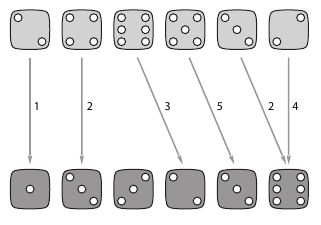
\includegraphics[scale=1]{pics/kubiki}
\caption{Две линии из шести игральных кубиков, с соответственными частичными суммами.}
\label{pic:kubiki}
\end{figure}

По построению, разница $\alpha_m-\beta_{m'}\ge 0$ не превышает $n-1$ 
(если $\alpha_m-\beta_{m'}\ge n$, то индекс $m'$ не максимален).
Если какая-то из разниц $\alpha_m-\beta_{m'}$ равна $0$, то задача решена --- в этом случае, взяв $j=s=1$, $k=m$ и $t=m'$, получим два начальных сегмента с одинаковыми суммами.
Если же ни одна из разниц $\alpha_m-\beta_{m'}$ не равна $0$, то все $n$ разниц 
$\alpha_m-\beta_{m'}$ лежат в множестве $\{1,\dots,n-1\}$ и, значит, две из них равны.
Предположим, что это $\alpha_p-\beta_{p'}$ и $\alpha_q-\beta_{q'}$.
Но тогда 
\[\sum_{i=p+1}^qa_i=\sum_{i=p'+1}^{q'}b_i.\]
--- снова победа.

Ну ведь хитр\'{о}! --- возражения не принимаются.

На рисунке есть только одна пара совпадающих разностей (обе равны 2), а именно $p=2$, $q=5$, $p'=2$ и $q'=6$;
вот соответственные подстроки с равными суммами:
\[a_3+a_4+a_5=6+5+3=3+2+3+6=b_3+b_4+b_5+b_6.\]

\begin{addedbytheeditors}
У этой идеи есть и другие применения; иногда неожиданные как например следующий результат \cite{petrunin}:
\textit{Если $\tilde M\to M$ --- $n$-листное локально-изометрическое накрытие компактного риманова многообразия $M$, то $\mathrm{diam}\, \tilde M\le n\cdot \mathrm{diam}\, M$}, где $\mathrm{diam}\, M$ обозначает \textit{диаметр $M$}, то есть максимальное расстояние между парой точек в $M$.

\textbf{Редакторам:} Надо исправить картинку --- третья стрелка слева должна указывать на 5-ку. 
\end{addedbytheeditors}


{
\small

\printindex

}

{

\sloppy

\printbibliography[heading=bibintoc]


\fussy

}

\newpage

{

\tableofcontents

}

\end{document}
